\textbf{VANET (Vehicle Ad Hoc Network)}とは, モバイル
アドホックネットワーク技術を車両間通信に応用したネットワークである
\cite{adhoc,vanet}. VANETは, 車両間の通信(Vehicle-to-Vehicle, 
\textbf{V2V}), および車両インフラ(路側機やドローン)間通信
(Vehicle-to-Infrastructure, \textbf{V2I})\cite{drone}で構成され, 
固定されたインフラに依存せず, ノード同士が自律的に
通信ネットワークを形成する. VANETでは, 車両間の距離が
無線通信の範囲を超えることが一般的であるため, 図\ref{fig:vanet}のように, 
データを送信元から宛先まで直接通信できない場合に, 
中継ノードを経由してデータを転送する. このような通信を
\textbf{マルチホップ通信}という.

\begin{figure}
  \centering
  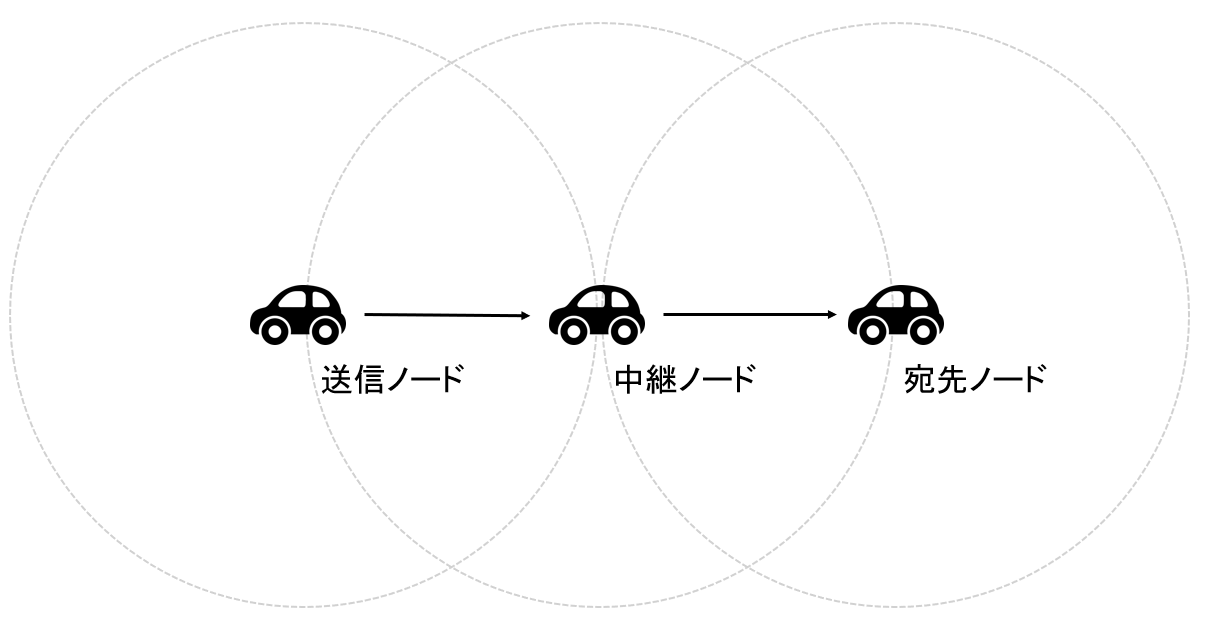
\includegraphics[scale=0.6]{figures/vanet.png}
  \caption{マルチホップ通信\cite{shinato}}
  \label{fig:vanet}
\end{figure}

VANETには次の5つの特徴がある.\\[0.5em]
\noindent\textbf{(1) 十分な電力供給}\\
\indent VANETを利用する際, 車両は走行していることを前提とするため, 
スマートフォンのような電池駆動のモバイルデバイスとは異なり, 
電力の制約は無視できる. したがって, 長時間の稼働や
高い通信レートの実現が可能であると仮定する. とはいえ, 高性能な
通信モジュールやセンサーを多数搭載する場合, 車両の
エネルギー効率に影響を与える可能性が考えられるため, 依然として
効率的なデバイス設計は求められる.\\[1em]
\noindent\textbf{(2) 位置情報の取得}\\
\indent 車両はGPSを搭載しているため, 自身の位置情報を取得できる.\\[1em]
\noindent\textbf{(3) ネットワークトポロジーの急速な変化}\\
\indent 無線通信では,ノード同士が直接的に通信可能であることを
\textbf{接続している}といい, この接続状態をもとにネットワーク全体の構造が形成される. 
このネットワーク構造を\textbf{ネットワークトポロジー}という. 
VANETでは通信するノードを車両と想定しているため, 
移動速度の速いノードが動的にネットワークを形成する. 
そのため, 接続の頻繁な確立と切断が発生し, 
ネットワークトポロジーは急速に変化する. \\[1em]
\noindent\textbf{(4) 移動の制約}\\
\indent 車両の動きは道路や建造物などの物理的構造に従う.\\[1em]
\noindent\textbf{(5) 安全に関する情報のリアルタイム性}\\
\indent 交通事故や道路状況に関する情報を即座に共有するためには, 
低遅延かつ信頼性の高い通信が求められる.\\

VANETは, 車両間通信や車両インフラ間通信を実現するための
優れた技術としてのポテンシャルを有する一方で, 
いくつかの課題も抱えている.
その中でも, セキュリティに関する課題は, VANETを安全かつ信頼性の
高いシステムとして運用する上で最も重要な課題の1つとなっている
\cite{vanet-challenge,vanet-security}.\\

